\documentclass[11pt,notes=hide,aspectratio=169,mathserif]{beamer}

% PACKAGES
\usepackage{graphics}  % Support for images/figures
\usepackage{graphicx}  % Includes the \resizebox command
\usepackage{tikz}      % For flowcharts
\usetikzlibrary{arrows.meta, positioning} % Libraries for TikZ


\usepackage{url}	   % Includes \urldef and \url commands
\usepackage{natbib}
\usepackage{bibentry}  % Includes the \nobibliography command
\usepackage{verbatim}  %Supports comments
\usepackage{booktabs} %Supports \toprule, \bottomrule, etc in tables
\usepackage{etoolbox}  %Supports toggle commands
\usepackage{datetime}
\usepackage{bm}	%Supports bold math \bm
%the LaTeX standard:
\usepackage{cmbright}
\setbeamerfont{frametitle}{family=\fontfamily{cmbr}\selectfont,size=\Large}
\fontencoding{OT1}\fontfamily{cmbr}\selectfont

% PACKAGES (that should already be included by your LyX document settings)
\usepackage{amsfonts}  % Lots of stuff, including \mathbb 
\usepackage{amsmath}   % Standard math package
\usepackage{amsthm}    % Includes the comment functions
\usepackage{subcaption}

% CUSTOM DEFINITIONS
\def\newblock{} %Get beamer to cooperate with BibTeX
\linespread{1.2}

% IDENTIFYING INFORMATION
\title[class]{ECON 326: Economics of Developing Countries \\ TA Session 3}
\author[vaidehi's class ]{Vaidehi Parameswaran (Northwestern Econ)}
\date{\monthname[\the\month] \the\year}

% THEMATIC OPTIONS
%\setbeamercovered{transparent}
\usetheme{metropolis}
\definecolor{mycolor}{RGB}{48,7,144} 
\setbeamercolor{frametitle}{bg=mycolor, fg=white} % Frame title color
\setbeamercolor{title separator}{fg=mycolor} 
\setbeamercolor{progress bar}{fg=mycolor} 
\beamertemplatenavigationsymbolsempty
\setbeamertemplate{footline}[frame number]{}
\setbeamertemplate{itemize item}{\small\raisebox{1pt}{\textcolor{mycolor}{$\blacktriangleright$}}}
\setbeamertemplate{itemize subitem}{\footnotesize\raisebox{1pt}{\textcolor{mycolor}{$\triangleright$}}}
\setbeamertemplate{itemize subsubitem}{\tiny\raisebox{1pt}{\textcolor{mycolor}{$\triangleright$}}}

% BACKUP SLIDE NUMBERING
\usepackage{appendixnumberbeamer}

\begin{document}

%---------------------------------------------------------------------
\begin{frame}[plain]
\titlepage
\end{frame}
%---------------------------------------------------------------------

%\section{Overview}

%---------------------------------------------------------------------
\begin{frame}{Today's Agenda}
Evidence on Cash Transfer Programs
\begin{itemize}
\item Effects on Child Health: \href{https://www.aeaweb.org/articles?id=10.1257/0002828041302109}{\textcolor{blue}{Gertler (2004)}}
\item Conditional Cash Transfers vs Unconditional Cash Transfers
\item Effects on Education: \href{https://academic.oup.com/qje/article-abstract/126/4/1709/1922509?login=false}{\textcolor{blue}{Baird, McIntosh \& Ozler (2011)}}
\end{itemize}
\end{frame}
%---------------------------------------------------------------------



\section*{\href{https://www.aeaweb.org/articles?id=10.1257/0002828041302109}{\textcolor{blue}{Gertler (2004)}} \\[5mm] 
\textnormal{\small{Do Conditional Cash Transfers Improve Child Health? Evidence from PROGRESA's Control Randomized Experiment}}}

%---------------------------------------------------------------------
\begin{frame}{Overview}
\begin{itemize}
\item Paper evaluates the impact of a large-scale RCT in Mexico 
\pause \item Conditional Cash Transfer (CCT) Program called PROGRESA in Mexico
\item Preview of result: \pause CCTs improve child health significantly 
\pause \item Suggestive that CCTs are effective and can be used to achieve equality of opportunity 
\end{itemize}
\end{frame}
%---------------------------------------------------------------------

%---------------------------------------------------------------------
\begin{frame}{PROGRESA}
\begin{itemize}
\item A CCT program in Mexico established in 1997 to address needs of extreme poverty
\pause \item What are the conditions?
\begin{itemize}
    \pause \item Children of age 0-23 get immunised and visit nutrition monitoring clinics every two months 
    \pause \item Children of age 24-60 months visit nutrition monitoring clinics every four months 
    \pause \item Pregnant and lactating mothers visit clinics to receive care 
    \pause \item Other family members visit clinics for physical check-ups
    \pause \item All adult family members participate in regular meetings to discuss health and nutrition
\end{itemize}
\pause \item If conditions are met, household receives cash transfer every two months
\pause \item Sizeable cash transfer - roughly 20-30\% of household income
\end{itemize}
\end{frame}
%---------------------------------------------------------------------

%---------------------------------------------------------------------
\begin{frame}{PROGRESA}
\begin{itemize}
\item So what does the program incentivise? \pause Using these health clinics
\pause \item Who is eligible? \pause Poor households in underserved communities
\pause \item Over first three years, extended benefits to 2.6 million families in 50,000 villages 
\pause \item which is 40\% of all rural families and 10\% of all families in Mexico 
\pause \item Budgetary and logistical constraints led the government to roll out program over a period of time 
\pause \item So the government randomly selected 320 villages to receive the program in 1998 and 185 villages to receive the program in 2000 
\pause \item Led to clear treatment and control groups 
\pause \item (without some usual ethical concerns)
\end{itemize}
\end{frame}
%---------------------------------------------------------------------

%---------------------------------------------------------------------
\begin{frame}{Empirical Strategy}
\begin{itemize}
\item Estimating equation: $Y_i =  \theta + \rho Z_i + u_i $
\pause \item $Z_i$ denoted treatment status 
\begin{itemize}
    \pause \item $Z_i = 1$ if village $i$ received PROGRESA in 1998 (Treatment group)
    \pause \item $Z_i = 0$ if village $i$ received PROGRESA in 2000 (Control group)
\end{itemize}
\pause \item Reduced-form equation to estimate the effect of being randomly assigned to treatment group 
\pause \item This captures an Intent To Treat (ITT) effect. Why? 
\pause \item The sample is restricted to eligible households only
\begin{itemize}
    \pause \item Exclude non-poor households in the experimental villages, about 22\%
\end{itemize}
\pause \item 2 rounds of data collection
\begin{itemize}
    \pause \item Baseline in early 1998. What's this data used for? 
    \pause \item Endline in 2000
\end{itemize}
\end{itemize}
\end{frame}
%---------------------------------------------------------------------

%---------------------------------------------------------------------
\begin{frame}{Empirical Strategy}
\begin{itemize}
    \item Very high compliance rate - 93\%
    \pause \item Who are the compliers here?
    \pause \item Who are the non-compliers here?
    \pause \item Local Average Treatment Effect (LATE) is given by $\frac{\text{ITT}}{\text{Compliance Rate}}$
    \pause \item So LATE and ITT are very similar in this case
    \pause \item Let's focus on $\rho$
\end{itemize}
\end{frame}
%---------------------------------------------------------------------

%---------------------------------------------------------------------
\begin{frame}{Balance Test}
\begin{itemize}
\item Ideally want health outcomes and other household characteristics to be balanced across treatment and control groups. Why?
\pause \item If not, there could be something systematically different between the two groups that could be driving the results 
\pause \item In practice, it is normal to have slight differences in means 
\begin{itemize}
    \pause \item Because people are different in real life 
    \pause \item Look at the p-values of the difference in means 
    \pause \item Tells us the likelihood of observing differences as large as the ones we observe by chance 
\end{itemize}
\end{itemize}
\end{frame}
%---------------------------------------------------------------------

%---------------------------------------------------------------------
\begin{frame}{Balance Test}
\begin{figure}
\centering
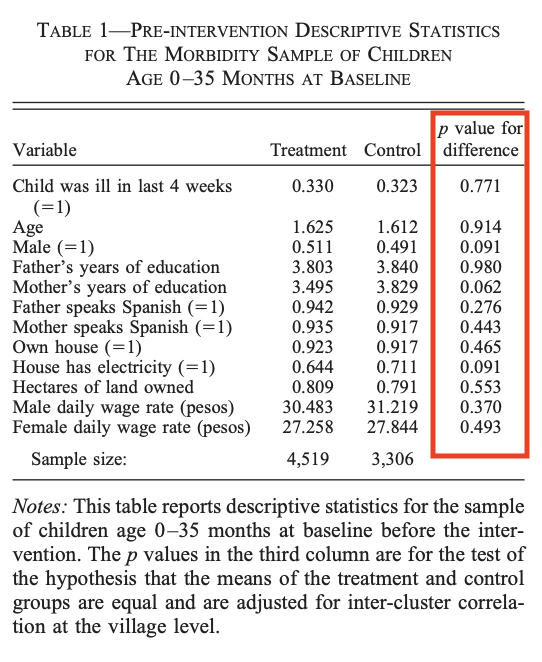
\includegraphics[width=0.4\textwidth]{inputs/table1.png}
\end{figure}
\end{frame}
%---------------------------------------------------------------------

%---------------------------------------------------------------------
\begin{frame}{Results}
\begin{figure}
\centering
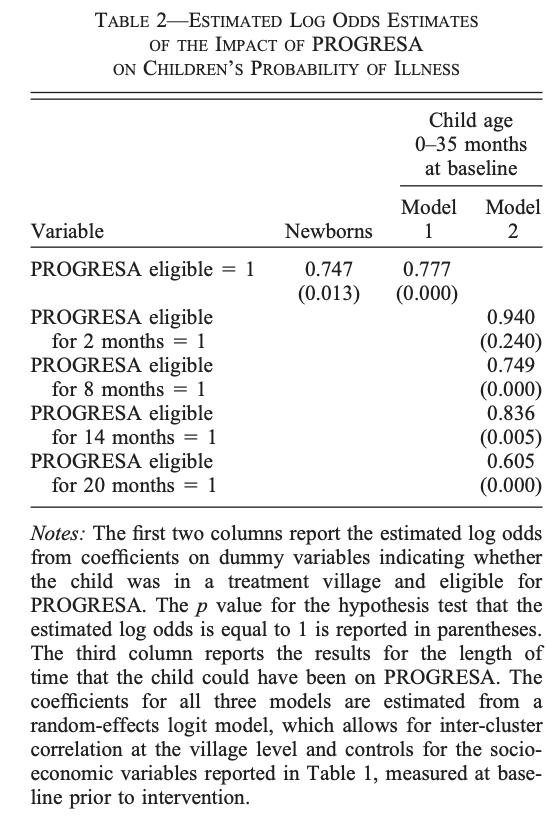
\includegraphics[width=0.28\textwidth]{inputs/table2.png}
\end{figure}
\begin{itemize}
\item Treatment newborns 25.4\% less likely to be reported as having been ill in the previous month
\end{itemize}
\end{frame}
%---------------------------------------------------------------------

%---------------------------------------------------------------------
\begin{frame}{Results}
\begin{figure}
\centering
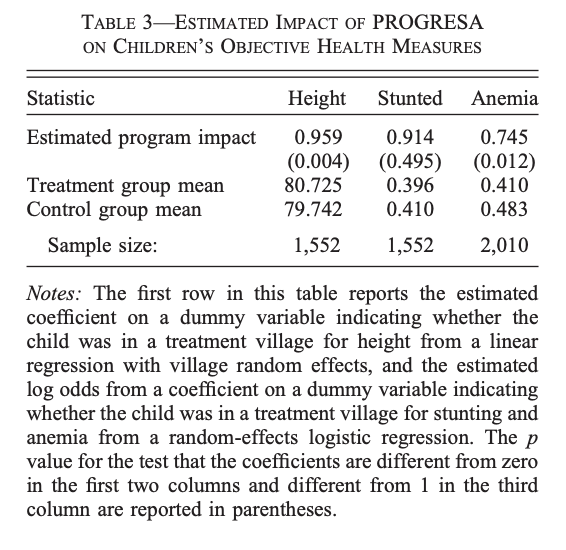
\includegraphics[width=0.4\textwidth]{inputs/table3.png}
\end{figure}
\begin{itemize}
\item Increase in children's height 
\item Control group more likely to be stunted (8.6\%) and more likely to be anaemic (25.5\%)
\end{itemize}
\end{frame}
%---------------------------------------------------------------------

%---------------------------------------------------------------------
\begin{frame}{Open Questions}
\begin{itemize}
\item Long-term impacts?
\item Was it the \textbf{conditional} or the \textbf{cash} part of the CCT that matters? 
\begin{itemize}
    \pause \item What would be the effect of a UCT?
\end{itemize}
\end{itemize}
\end{frame}
%---------------------------------------------------------------------

\section*{CCTs vs UCTs}

%---------------------------------------------------------------------
\begin{frame}{Conditional Cash Transfers - Pros and Cons}
\begin{itemize}
\item Pros
\begin{itemize}
    \pause \item Incentivises certain behaviours that can potentially correct market failures 
    \pause \item Can be used to target specific outcomes 
    \pause \item Politically palatable
\end{itemize}
\item Cons
\begin{itemize}
    \pause \item Can be paternalistic 
    \pause \item Can be expensive to monitor compliance
\end{itemize}
\end{itemize}
\end{frame}
%---------------------------------------------------------------------

%---------------------------------------------------------------------
\begin{frame}{Why UCTs might be better}
\begin{itemize}
    \pause \item Easier to implement
    \pause \item Theoretical default - people are rational 
\end{itemize}
\end{frame}
%---------------------------------------------------------------------

\section*{\href{https://academic.oup.com/qje/article-abstract/126/4/1709/1922509?login=false}{\textcolor{blue}{Baird, McIntosh \& Ozler (2011)}} \\[5mm] 
\textnormal{\small{Cash or Condition? Evidence from a Cash Transfer Experiment}}}

%---------------------------------------------------------------------
\begin{frame}{Overview}
\begin{itemize}
\item Paper compares the effects of a UCT and a CCT in Malawi in 2007-2009
\pause \item Interested in effects on education as opposed to health (as in Gertler 2004)
\pause \item Provided cash transfers to households with school-age girls (ages 13 - 22)
\begin{itemize}
    \pause \item This group was at risk of dropping out 
    \pause \item Objective was to keep them in school
\end{itemize}
\pause \item CCT arm was conditional on school attendance - payment made if attendance $>$ 80\%
\pause \item UCT arm was unconditional - payment made regardless of attendance
\end{itemize}
\end{frame}
%---------------------------------------------------------------------

%---------------------------------------------------------------------
\begin{frame}{RCT Design}
\begin{itemize}
\item Unit of randomisation - Enumeration Area (EA)
\pause \item 176 EAs selected from different strata - urban, rural, far rural 
\pause \item Randomly divided into equal size groups of treatment and control 
\pause \item 88 treatment EAs further divided 
\begin{itemize}
    \pause \item 46 EAs for the CCT arm
    \pause \item 27 EAs for the UCT arm 
    \pause \item 15 EAs received no cash treatment
\end{itemize}
\pause \item In each EA, a percentage of baseline school girls was randomly selected to participate 
\pause \item Cash transfer made to both the girls and the parent - amount varied by EA 
\end{itemize}
\end{frame}
%---------------------------------------------------------------------

%---------------------------------------------------------------------
\begin{frame}{Data Collection}
\begin{itemize}
\item Baseline data in 2007 - 2008 before participation was sought 
\pause \item Follow up surveys in 2008 - 2009 and in 2010 
\pause \item Use household surveys, school surveys, school ledgers, interviews, test score data 
\end{itemize}
\end{frame}
%---------------------------------------------------------------------

%---------------------------------------------------------------------
\begin{frame}{Balance Test}
\begin{figure}
\centering
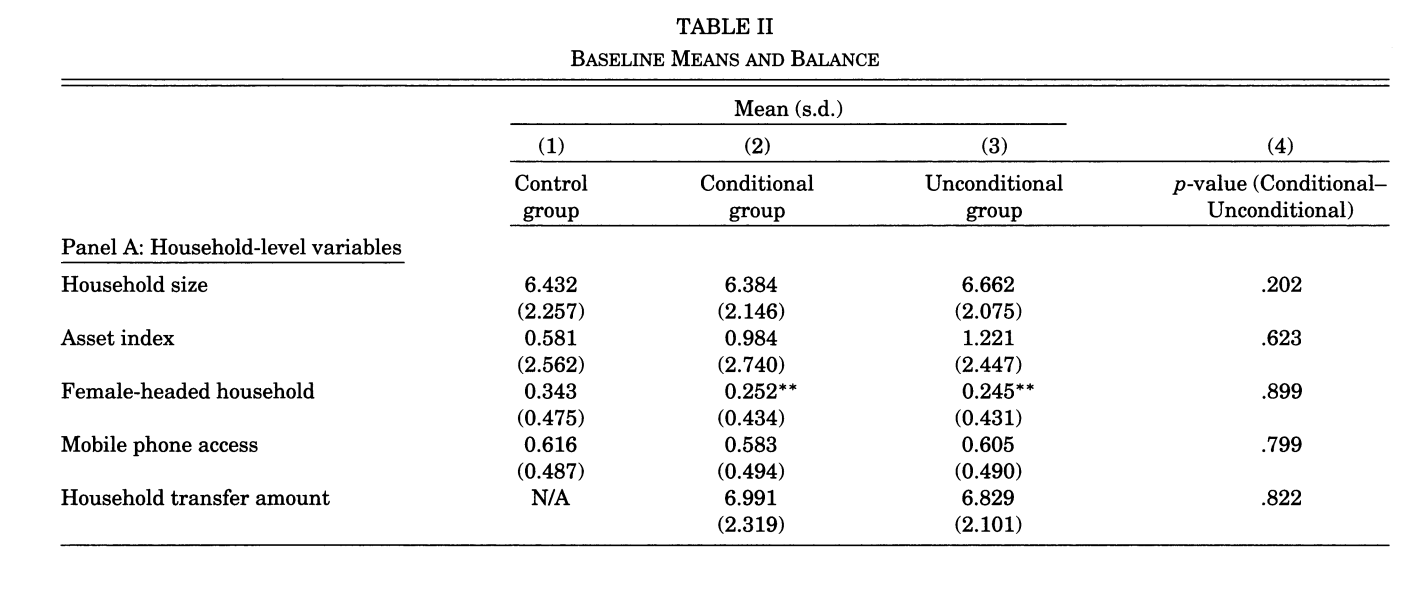
\includegraphics[width=0.5\textwidth]{inputs/table4.png}\\
\vspace{0.0cm} 
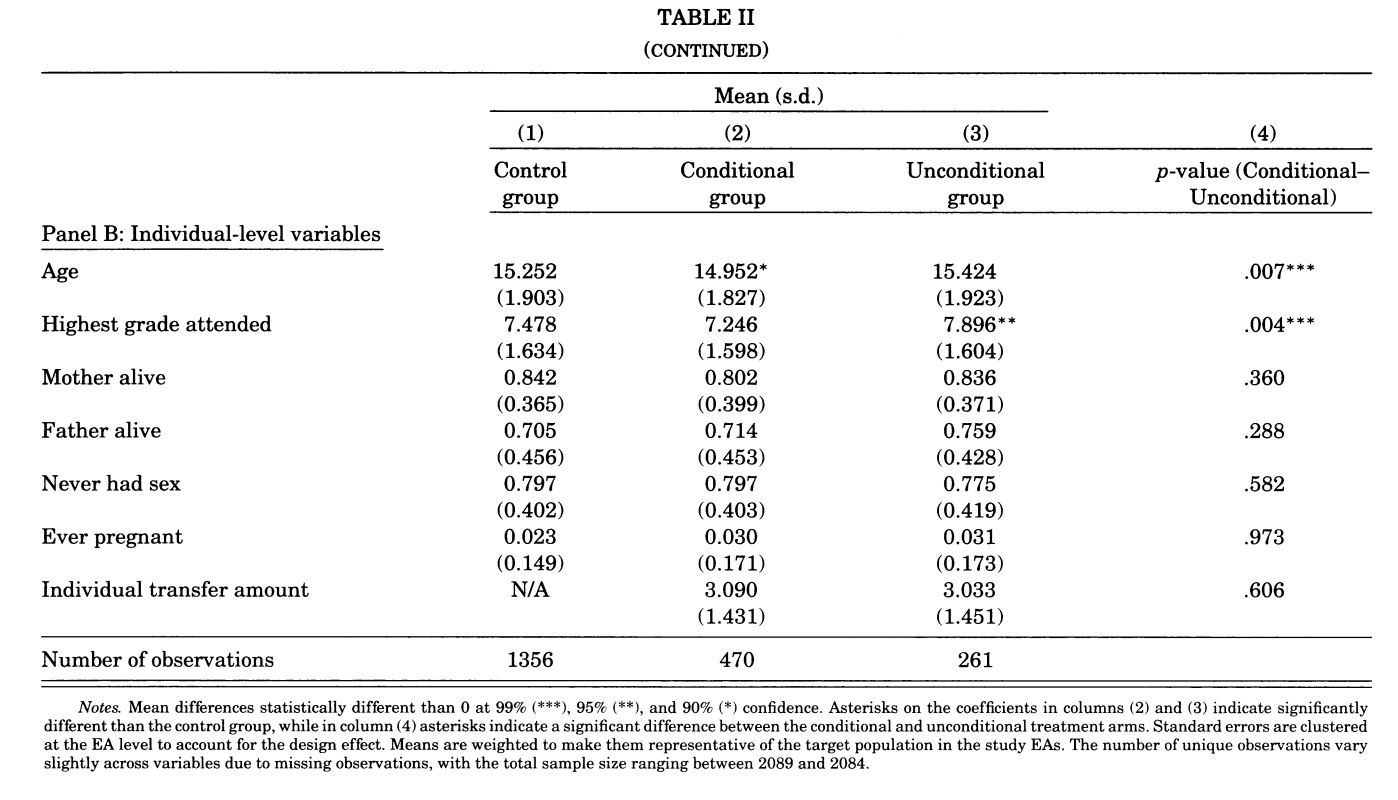
\includegraphics[width=0.5\textwidth]{inputs/table5.png}
\end{figure}
\end{frame}
%---------------------------------------------------------------------

%---------------------------------------------------------------------
\begin{frame}{Results: Schooling Outcomes}
Student-reported school enrollment imply that UCTs are better ...
\begin{figure}
\centering
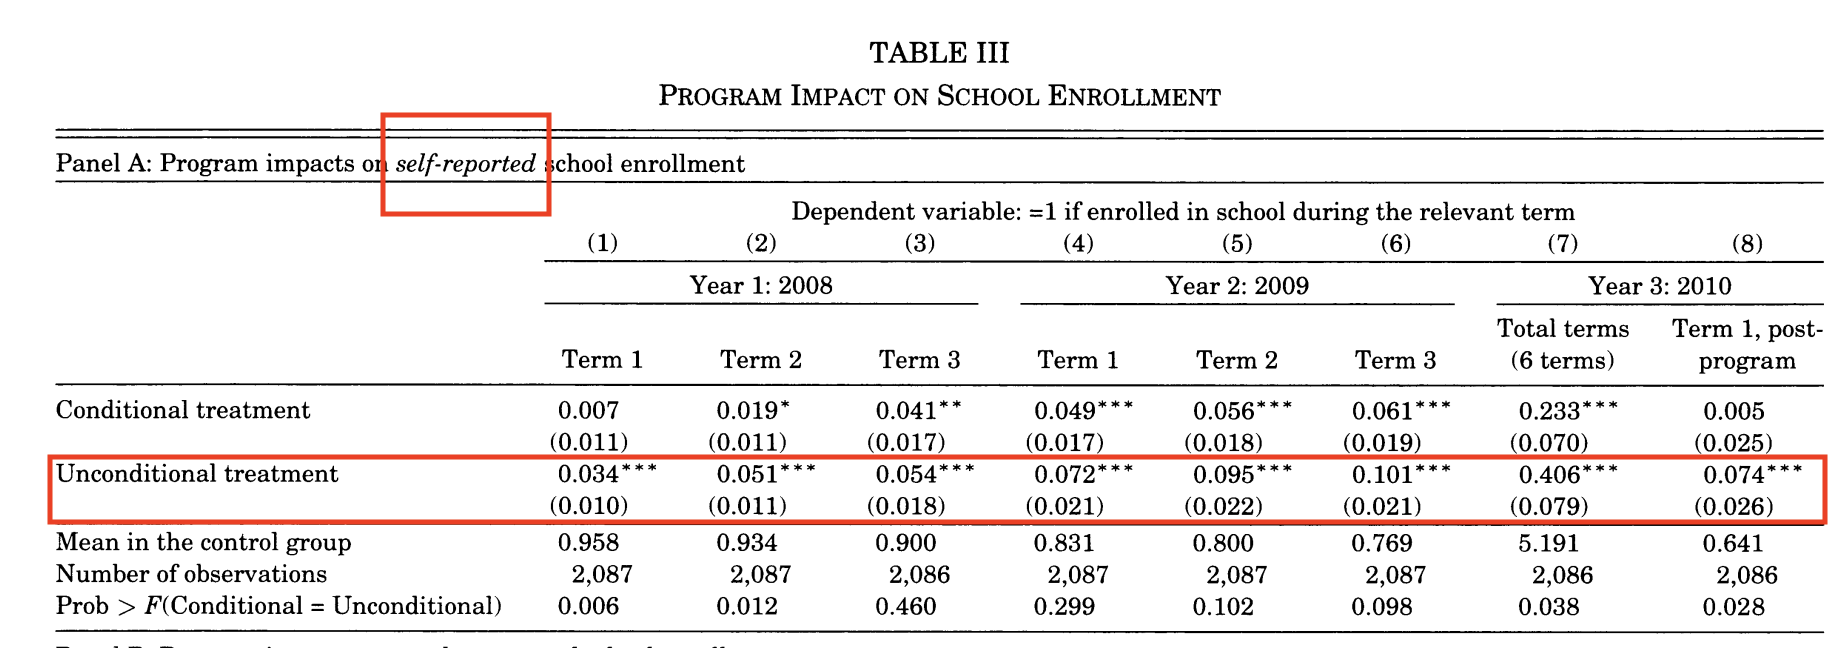
\includegraphics[width=0.5\textwidth]{inputs/table6.png}
\end{figure}
\end{frame}
%---------------------------------------------------------------------

%---------------------------------------------------------------------
\begin{frame}{Results: Schooling Outcomes}
Teacher-reported school enrollment imply that CCTs are better ...
\begin{figure}
\centering
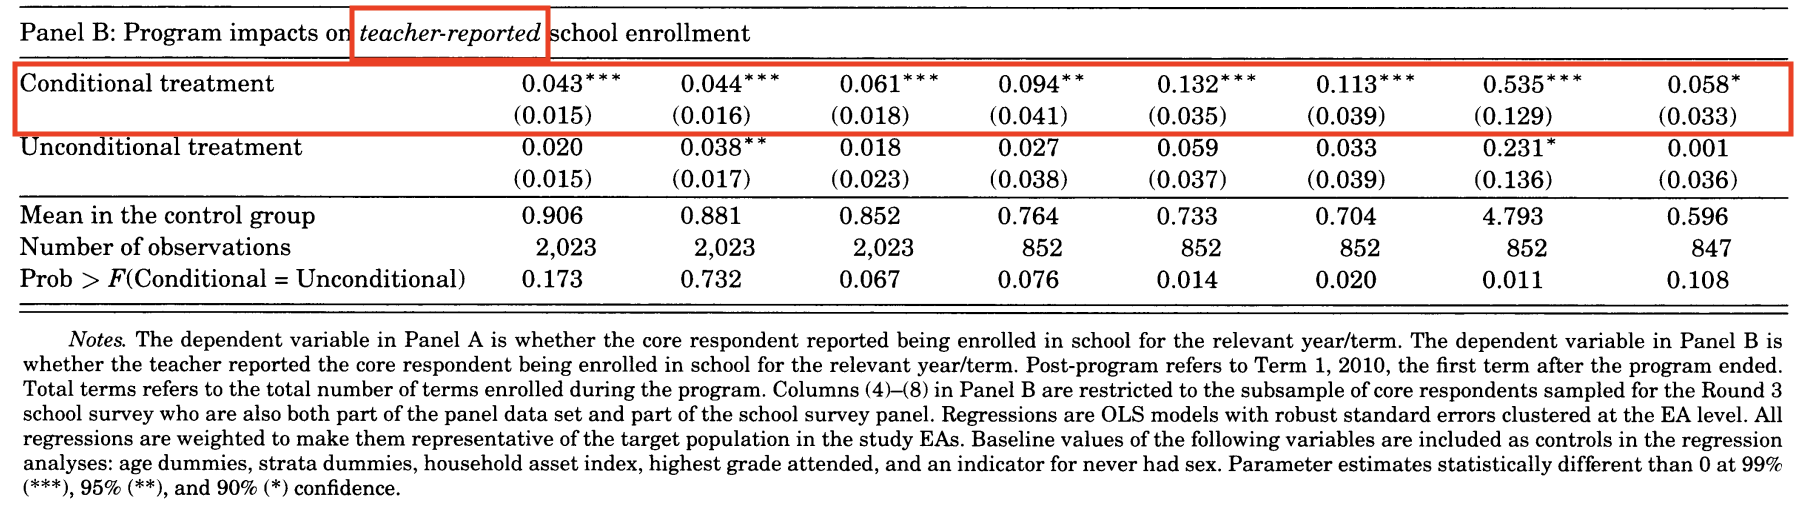
\includegraphics[width=0.5\textwidth]{inputs/table7.png}
\end{figure}
\pause So it seems to depend on who you ask. \\
\pause But the authors believe that teacher-reported data is less likely to be biased. 
\end{frame}
%---------------------------------------------------------------------

%---------------------------------------------------------------------
\begin{frame}{Results: Attendance}
Among those who stay in school, school records favour CCTs over UCTs
\begin{figure}
\centering
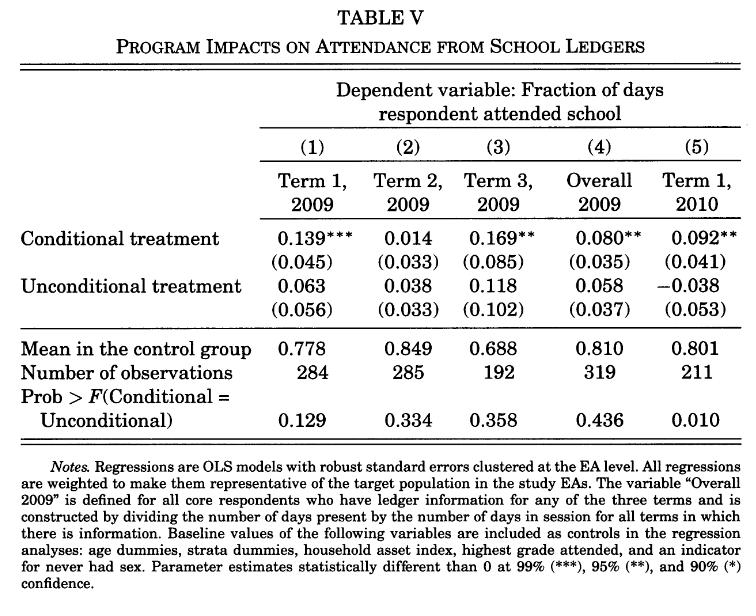
\includegraphics[width=0.5\textwidth]{inputs/table8.png}
\end{figure}
\end{frame}
%---------------------------------------------------------------------

%---------------------------------------------------------------------
\begin{frame}{Results: Test Scores}
Test scores are also higher in the CCT group
\begin{figure}
\centering
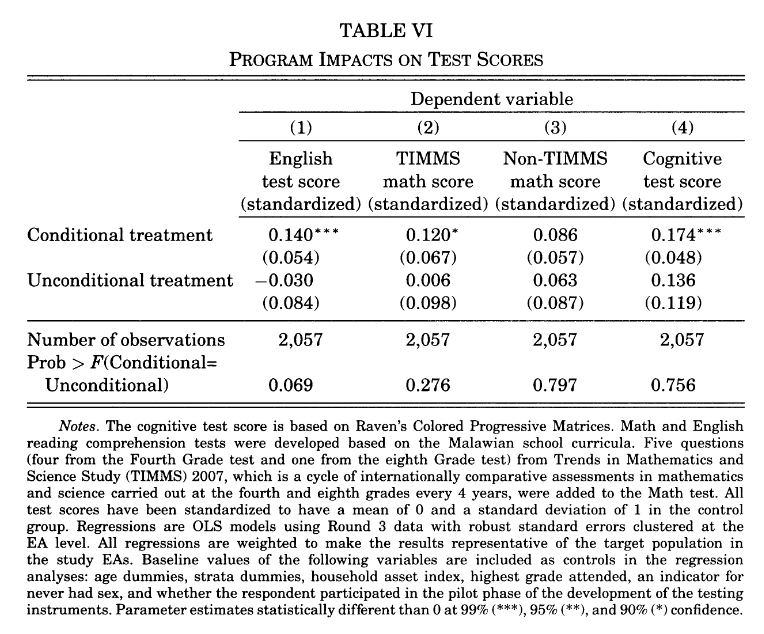
\includegraphics[width=0.5\textwidth]{inputs/table9.png}
\end{figure}
\end{frame}
%---------------------------------------------------------------------

%---------------------------------------------------------------------
\begin{frame}{Results: Long-term Outcomes}
\begin{figure}
\centering
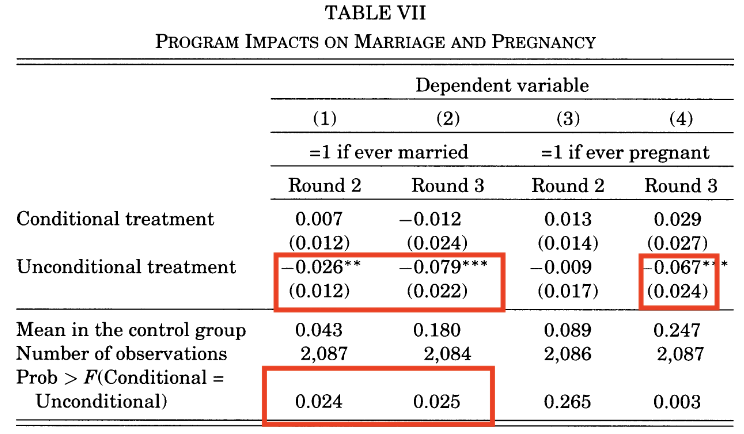
\includegraphics[width=0.5\textwidth]{inputs/table10.png}
\end{figure}
\end{frame}
\begin{frame}{Results: Long-term Outcomes}
\begin{itemize}
    \item Marriage rates unchanged in CCT group but significantly lower in UCT group
    \pause \item How to reconcile that CCT boosted schooling outcomes but only UCT reduced marriage rates?
    \begin{itemize}
        \pause \item Two channels for schooling to affect marriage 
        \pause \item Through the CCT arm, dropouts averted 
        \pause \item Through the UCT arm, girls dropped out but income effect delayed marriage 
        \pause \item The second group is larger than the first group in this study 
    \end{itemize}
\end{itemize}
\end{frame}
%---------------------------------------------------------------------

%---------------------------------------------------------------------
\begin{frame}{Conclusion: No Clear Winner}
\begin{itemize}
\item CCTs increased enrollment and regular attendance for those in school more than the UCT
\pause \item UCTs substantially lowered teenage pregnancy and marriage rates 
\pause \item CCTs more cost-effective at improving schooling outcomes - they use different payment amounts to learn this 
\pause \item So which program to choose may depend on the level of compliance 
\pause \item Ultimately, some of these individuals need income support and are vulnerable
\pause \item ``while CCT programs may be more effective than UCTs in obtaining the desired behaviour change, they can also undermine the social protection dimension of cash transfer programs''
\end{itemize}
\end{frame}
%---------------------------------------------------------------------

%---------------------------------------------------------------------
\begin{frame}
\begin{center}{\LARGE See you next time!}\end{center}
\end{frame}
%---------------------------------------------------------------------


\end{document}